\documentclass[12pt, a4paper]{article}

% ---- Packages -----------------------------------------------
\usepackage[margin=1in]{geometry}
\usepackage{amsmath, amssymb}
\usepackage{booktabs}
\usepackage{tabularx}
\usepackage{graphicx}
\usepackage[labelfont=bf, font=small, justification=justified]{caption}
\usepackage[numbers, compress]{natbib}
\usepackage[colorlinks=true, linkcolor=blue, citecolor=blue, urlcolor=blue]{hyperref}
\usepackage{parskip}
\usepackage[T1]{fontenc}

% Supplementary figure counter
\newcounter{suppfig}
\renewcommand{\thesuppfig}{S\arabic{suppfig}}

% =============================================================
\begin{document}

% ---- Title block ----------------------------------------------
\begin{center}
{\Large\bfseries Supplementary Material}

\vspace{0.5cm}

{\large A schedule-driven framework for estimating infectious
disease importation risk at mass gathering events: the 2026 FIFA
World Cup as a case study}

\vspace{0.5cm}

Jose L. Herrera-Diestra$^{1,*}$, Nyall Jamieson$^{2}$, Mallory J. Harris$^{2,3,4}$, Kaiming Bi$^{5}$, Martial L. Ndeffo-Mbah$^{6}$,  Melissa Zeynep Ertem$^{7}$, Amera Al-Amery$^{8}$

\vspace{0.3cm}

{\small
$^{1}$ Department of Mathematics, Tarleton State University, Stephenville, TX 76402, USA\\
$^{2}$ Department of Integrative Biology, University of Texas at Austin, Austin, TX 78712, USA\\
$^{3}$ Department of Biology, University of Maryland, College Park, MD 20742, USA\\
$^{4}$ University of Maryland Institute for Health Computing, North Bethesda, MD 20852, USA\\
$^{5}$ Department of Management, Policy and Community Health, School of Public Health, The University of Texas Health Science Center at Houston, Houston, TX 77030\\
$^{6}$ Department of Veterinary Integrative Biosciences, College of Veterinary Medicine \& Biomedical Sciences, Texas A\&M University, College Station, TX 77843, USA\\
$^{7}$ Thomas J. Watson College of Engineering, State University of New York at Binghamton, NY, 13850, USA\\
$^{8}$ Department of Computer Information Systems, Jordan University of Science and Technology, Irbid, Jordan\\
$^{*}$ Corresponding author.
E-mail: \href{mailto:jherreradiestra@tarleton.edu}{jherreradiestra@tarleton.edu}
}
\end{center}

\vspace{0.5cm}

\setcounter{suppfig}{0}

% ---- Appendix A ---------------------------------------------
\subsection*{Appendix A. Mathematical specification of travel flow
estimates $N_{c,v}$}

\subsubsection*{A.1 Notation}

\begin{center}
\small
\begin{tabular}{p{2.2cm} p{10cm}}
\toprule
\textbf{Symbol} & \textbf{Definition} \\
\midrule
$c$ & Source country ($c = 1,\ldots,C$) \\
$v$ & US venue city ($v = 1,\ldots,11$) \\
$A_c$ & June 2024 COR arrivals from country $c$ to the US
        (I-94 programme, CBP) \\
$T_{c,v}$ & Mean June passengers from country $c$ to US city $v$,
        averaged over June 2023--2025 (BTS T-100 Form 41 data) \\
$f_{c,v}^{T}$ & T-100 routing fraction: share of country $c$'s
        US-bound passengers landing at city $v$ (see A.2).
        By construction $\sum_{v} f_{c,v}^{T} = 1$. \\
$\phi_c$ & Country-specific 2026 growth factor (see A.3) \\
$g_c$ & Background (non-WC) trend component of $\phi_c$,
        representing non-WC travel growth from 2024 to 2026 \\
$m_{c,v}$ & Number of group-stage matches that country $c$
        plays at US venue $v$ \\
$M_c$ & Total group-stage matches for country $c$ across all WC venues ($M_c = 3$ for all qualified teams) \\
$\omega_{c,v}$ & Schedule-driven routing fraction for WC fans
        from country $c$ to US venue $v$ (see A.4) \\
$N_{c,v}$ & Projected June 2026 arrivals from country $c$
        to venue city $v$ (model-tier specific) \\
\bottomrule
\end{tabular}
\end{center}

\subsubsection*{A.2 T-100 routing fraction $f_{c,v}^{T}$}

The T-100 routing fraction gives the proportion of country $c$'s
US-bound passengers that land at each venue city $v$:
\[
  f_{c,v}^{T} = \frac{T_{c,v}}{\displaystyle\sum_{v'=1}^{11} T_{c,v'}}
\]
where $T_{c,v}$ is the mean number of June passengers from country
$c$ to US city $v$ over 2023--2025 (BTS T-100 Form 41 data). By
construction, $\sum_{v} f_{c,v}^{T} = 1$ for every country $c$.
These fractions are held fixed across all three model tiers; only
the total volume $A_c \cdot \phi_c$ changes between M1, M2, and M3.

\subsubsection*{A.3 Growth factor $\phi_c$ and its components}

The growth factor
\[
  \phi_c = \frac{V_{c,2026}}{V_{c,2024}}
\]
scales June 2024 baseline arrivals to projected June 2026 levels,
where $V_{c,t}$ denotes projected total June visitors from country
$c$ in year $t$. Three country classes are distinguished:

\begin{enumerate}
  \item \textbf{Top-12 inbound markets} (Australia, Brazil, Canada,
    China, France, Germany, India, Italy, Japan, Mexico, South Korea,
    UK) --- NTTO country-specific projections:
    \[
      \phi_c = \frac{A_{c,2026}^{\text{NTTO}}}{A_{c,2024}}
    \]
    The World Cup effect is already embedded in the NTTO forecast.
    The background (non-WC) trend component $g_c$ is derived from
    the pre-tournament NTTO trend excluding the tournament increment.

  \item \textbf{Other WC-qualified nations} --- a uniform World Cup
    growth factor is applied:
    \[
      \phi_c = \phi^{\text{WC}} = \frac{85{,}017}{72{,}390} = 1.174
    \]
    reflecting the aggregate fan-travel surge for smaller qualified
    markets (NTTO 2025 report). The background trend component is
    $g_c = \phi^{\text{bg}} = 1.077$, so the WC-specific fan
    increment is $\phi_c - g_c = 0.097$.

  \item \textbf{Non-qualified nations} --- no WC adjustment is made:
    \[
      \phi_c = g_c = \phi^{\text{bg}} = 1.077
    \]
    where $\phi^{\text{bg}}$ is the data-driven background growth
    rate estimated from COR and T-100 data (June 2023--2025).
    By construction, $\phi_c - g_c = 0$ for non-qualified countries.
\end{enumerate}

\subsubsection*{A.4 Schedule-driven routing fraction $\omega_{c,v}$}

For WC-qualified nation $c$, the fan stream is routed proportionally
to the share of its group-stage matches played at each US venue:
\[
  \omega_{c,v} = \frac{m_{c,v}}{M_c} = \frac{m_{c,v}}{3}
  \quad \text{(US venues only)}
\]
If country $c$ plays no matches at US venue $v$ then
$\omega_{c,v} = 0$. Matches played at Canadian or Mexican venues
contribute to $M_c$ but not to any US $\omega_{c,v}$, so:
\[
  \sum_{v=1}^{11} \omega_{c,v}
    = \frac{\text{(US matches of }c)}{3} \;\leq\; 1
\]
with strict inequality for nations playing one or more matches
outside the US. For non-qualified nations no WC fan stream exists
and $\omega_{c,v}$ is not used.

\subsubsection*{A.5 Travel decomposition for M3}

Model 3 separates total projected 2026 arrivals from country $c$
into a background stream and a WC fan stream:
\[
  N_c^{\text{WC}} = A_c \cdot \max\!\bigl(0,\;\phi_c - g_c\bigr)
  \qquad
  N_c^{\text{bg}} = A_c \cdot g_c
\]
Note that $N_c^{\text{WC}} + N_c^{\text{bg}} = A_c \cdot \phi_c$,
so the decomposition is exact and exhaustive. For non-qualified
countries $\phi_c = g_c$, giving $N_c^{\text{WC}} = 0$. For
typical WC-qualified nations the fan increment represents
approximately $(1.174 - 1.077)/1.174 \approx 8.3\%$ of total
projected 2026 arrivals.

\subsubsection*{A.6 Travel flow $N_{c,v}$ by model tier}

\paragraph{M1 --- Baseline.}
Raw June 2024 arrivals distributed by T-100 routing fractions;
no growth factor applied.
\[
  \boxed{N_{c,v}^{M1} = A_c \cdot f_{c,v}^{T}}
\]

\paragraph{M2 --- WC-adjusted.}
Projected 2026 arrivals (incorporating the full growth factor
$\phi_c$) distributed by T-100 routing fractions. All WC fan
travel is assigned to US cities regardless of whether matches
are played in Canada or Mexico.
\[
  \boxed{N_{c,v}^{M2} = A_c \cdot \phi_c \cdot f_{c,v}^{T}}
\]

\paragraph{M3 --- Schedule-driven.}
The background stream is T-100 routed; the WC fan stream is
routed by the match schedule:
\[
  \boxed{N_{c,v}^{M3}
    = \underbrace{N_c^{\text{bg}} \cdot f_{c,v}^{T}}_{\text{background stream}}
      \;+\;
      \underbrace{N_c^{\text{WC}} \cdot \omega_{c,v}}_{\text{WC fan stream}}
    = A_c \Bigl[
        g_c \cdot f_{c,v}^{T}
        + (\phi_c - g_c) \cdot \omega_{c,v}
      \Bigr]}
\]
For non-qualified nations $\phi_c = g_c$, so the fan stream
vanishes and $N_{c,v}^{M3} = A_c \cdot g_c \cdot f_{c,v}^{T}$.

\subsubsection*{A.7 Why $N_{c,v}^{M3} \leq N_{c,v}^{M2}$ for
US cities}

M2 routes the entire WC increment $(\phi_c - g_c)$ through T-100
fractions, which sum to 1 over US cities. M3 routes the same
increment through schedule fractions, which sum to $\leq 1$ over
US cities (strictly $<1$ whenever country $c$ plays matches in
Canada or Mexico). Therefore:
\[
  \sum_{v} N_{c,v}^{M3}
    = A_c \Bigl[
        g_c \underbrace{\sum_v f_{c,v}^T}_{=1}
        + (\phi_c - g_c)
          \underbrace{\sum_v \omega_{c,v}}_{\leq 1}
      \Bigr]
  \;\leq\;
  A_c \cdot \phi_c
    = \sum_v N_{c,v}^{M2}
\]
The gap equals the fan travel redirected to non-US WC venues
(Canada, Mexico), which is why the M3 US-city total lies below
M2 for all qualified nations with at least one non-US match.
Importation probability heatmaps for M1 and M2 are shown in
Supplementary Figures~S1 and S2; these complement the M3 heatmap
in Figure 1 and the three-model comparison in
Figure 2 of the main text.

\newpage

% ---- Appendix B ---------------------------------------------
\subsection*{Appendix B. Mathematical specification of the diaspora
network extension}

\subsubsection*{B.1 Notation}

\begin{center}
\small
\begin{tabular}{p{2.8cm} p{9.5cm}}
\toprule
\textbf{Symbol} & \textbf{Definition} \\
\midrule
$D_{c,v}$            & Number of US residents born in country $c$
                       living in metro area $v$
                       (ACS 5-year estimates 2019--2023, Table B05006) \\
$\mathrm{FB}_{v}$    & Total foreign-born population of metro area $v$
                       (row total of Table B05006) \\
$\kappa_{c,v}$       & Diaspora concentration index: share of metro
                       $v$'s foreign-born population born in country $c$ \\
$\Omega^A_{c,v,d}$   & Expected number of infected arrivals from $c$
                       at city $v$ that enter the co-national network
                       (Mechanism A) \\
$P^A(\geq 1)_{v,d}$  & Probability that at least one infected arrival
                       enters any co-national network in city $v$ \\
$v_{\text{match}}$   & WC venue city where country $c$ plays \\
$v_{\text{home}}$    & Diaspora hub city (may differ from
                       $v_{\text{match}}$) \\
$\omega_{c,v}$       & Schedule-driven routing fraction: share of
                       $c$'s group-stage matches played at US venue
                       $v$ (Appendix A.4); zero if $c$ does not play
                       at $v$ \\
$\Omega^B_{c,v_h,d}$ & Secondary seeding index for hub city $v_h$,
                       summed over all match venues where $c$ plays
                       (Mechanism B) \\
\bottomrule
\end{tabular}
\end{center}

\subsubsection*{B.2 Diaspora concentration index $\kappa_{c,v}$}

For each source country $c$ and venue metro area $v$:
\[
  \kappa_{c,v} = \frac{D_{c,v}}{\mathrm{FB}_{v}}
\]
$\kappa_{c,v} \in [0,1]$ measures how concentrated the country-$c$
community is \emph{within} the immigrant population of city $v$ ---
the relevant social network for co-national mixing. Summed over all countries of birth, $\sum_c \kappa_{c,v} = 1$ for each $v$; because the model includes only the source countries relevant to the five diseases, the $\kappa_{c,v}$ for the modeled countries sum to less than one in each city.

\subsubsection*{B.3 Mechanism A: local social mixing}

Let $X_{c,v,d} \sim \text{Poisson}(\lambda_{c,v,d})$ be the number
of infected arrivals from country $c$ at city $v$. Under the
proportional-mixing assumption, each arrival independently enters
the co-national network with probability $\kappa_{c,v}$. By the
Poisson thinning theorem \citep{Ross2010}, the thinned count is:
\[
  Y_{c,v,d} \sim \text{Poisson}(\lambda_{c,v,d} \cdot \kappa_{c,v})
\]
We define the community-weighted importation intensity:
\[
  \Omega^A_{c,v,d} = \lambda_{c,v,d} \cdot \kappa_{c,v}
    = \lambda_{c,v,d} \cdot \frac{D_{c,v}}{\mathrm{FB}_{v}}
\]
Because $Y_{c,v,d}$ values are independent Poisson random variables,
the city-level aggregate $\Omega^A_{v,d} = \sum_c \Omega^A_{c,v,d}$
is also a valid Poisson rate. The probability that at least one
infected arrival enters any co-national network in city $v$ is:
\[
  P^A(\geq 1)_{v,d} = 1 - e^{-\Omega^A_{v,d}}
\]
This is directly comparable to the main-model probability
$P(\geq 1)_{v,d} = 1 - e^{-\Lambda_{v,d}}$. Since
$\kappa_{c,v} \leq 1$ for all $c,v$, it follows that
$\Omega^A_{v,d} \leq \Lambda_{v,d}$ and therefore
$P^A(\geq 1)_{v,d} \leq P(\geq 1)_{v,d}$ always: the
diaspora-network probability is a lower bound on the arrival
probability, never exceeding it.

\subsubsection*{B.4 Mechanism B: diaspora return seeding}

US-resident diaspora members from country $c$ living in hub city
$v_{\text{home}}$ may travel domestically to $v_{\text{match}}$
(where country $c$ plays a US match), be exposed to infected
co-nationals within the local network that Mechanism A already
quantifies, and seed transmission upon return. The secondary seeding
index reuses the schedule-driven routing fraction $\omega_{c,v}$
(Appendix A.4) to restrict this pathway to venues where $c$ actually
plays, and the local exposure hazard $\Omega^A_{c,v,d}$ (Section B.3)
rather than the raw arrival rate $\lambda_{c,v,d}$:
\[
  \Omega^B_{c,\,v_{\text{home}},\,d}
    = \sum_{v_{\text{match}} \neq v_{\text{home}}}
      \omega_{c,\,v_{\text{match}}} \cdot \Omega^A_{c,\,v_{\text{match}},\,d}
      \cdot \kappa_{c,\,v_{\text{home}}}
\]
Because $\omega_{c,v} \leq 1$ and $\kappa_{c,v} \leq 1$ for all $c,v$,
and $\Omega^A_{c,v,d}$ is already a well-scaled Poisson rate
(Section B.3), $\Omega^B$ remains on the same scale as $\Omega^A$
rather than growing unboundedly, unlike a specification that instead
scales a raw diaspora headcount by an assumed match-attendance
probability. Summing over source countries gives the hub-city
aggregate:
\[
  \Omega^B_{v_{\text{home}},\,d} = \sum_c \Omega^B_{c,\,v_{\text{home}},\,d}
\]
and the corresponding probability that at least one returning
diaspora member seeds transmission in the hub city,
$P^B(\geq 1)_{v_{\text{home}},\,d} = 1 - e^{-\Omega^B_{v_{\text{home}},\,d}}$,
directly comparable to $P^A(\geq 1)_{v,d}$.

Because $\omega_{c,v_{\text{match}}} = 0$ whenever country $c$ does
not play a match at $v_{\text{match}}$ (Appendix A.4), $\Omega^B$ is
defined only for the subset of source countries that are both
WC-qualified and scheduled to play at a US venue --- 13 of the
source countries modeled here meet this condition. A country with
substantial $\Omega^A_{c,v,d}$ driven by routine background travel
to a city where it is not playing contributes zero to $\Omega^B$ at
that venue, since Mechanism B specifically models exposure acquired
while attending a match, not general travel; that country's local
risk is still fully captured by Mechanism A. This is a deliberate
scope restriction consistent with the mechanism's premise, not an
omission.

The match venue $v_{\text{match}}$ ranges over the 11 host cities, while the hub city $v_{\text{home}}$ ranges over both the 11 host cities and 15 major non-host metropolitan areas with large immigrant populations (drawn from the same ACS B05006 country-of-birth data), so that secondary seeding into non-venue cities
is captured. The 15 non-host hub metropolitan areas are Austin, Charlotte, Chicago,
Denver, Detroit, Las Vegas, Minneapolis, Orlando, Phoenix, Portland,
Sacramento, San Antonio, San Diego, Tampa, and Washington, DC.

\newpage

% ---- Table S1 -----------------------------------------------
\subsection*{Table S1. Sensitivity of expected importations to the mild-symptom travel probability $p_d$.}

Because $p_d$ enters the model multiplicatively
($\lambda_{c,v,d} = N_{c,v}\cdot\rho_d\cdot C_{c,d}/P_c\cdot p_d$),
fixing $\rho_d$ at its literature midpoint and varying $p_d$ produces
importation totals that scale exactly as $p_d/p_{\text{mid}}$. The
table below reports these relative values ($\Lambda_{\text{rel}}$,
normalised to 1.00 at $p_{\text{mid}}$) and the exact fold-change
$p_{\max}/p_{\min}$ for all five modelled diseases. Absolute 11-city
importation counts at each $p_d$ level are available in the
analysis code at \url{https://github.com/jdiestra1977/FIFA\_worldCup\_2026\_risk}.

\medskip
\begin{center}
\small
\begin{tabular}{lcccrrrr}
\toprule
\textbf{Disease} &
  $\boldsymbol{p_{\min}}$ &
  $\boldsymbol{p_{\text{mid}}}$ &
  $\boldsymbol{p_{\max}}$ &
  $\boldsymbol{\Lambda(p_{\min})}$ &
  $\boldsymbol{\Lambda(p_{\text{mid}})}$ &
  $\boldsymbol{\Lambda(p_{\max})}$ &
  \textbf{Fold} \\
\midrule
Dengue    & 0.30 & 0.50 & 0.70 & 29.70 & 49.50 & 69.29 & 2.3$\times$ \\
Malaria   & 0.10 & 0.30 & 0.50 &  6.08 & 18.25 & 30.42 & 5.0$\times$ \\
Measles   & 0.02 & 0.06 & 0.10 &  0.02 &  0.05 &  0.08 & 5.0$\times$ \\
Pertussis & 0.50 & 0.70 & 0.90 &  1.49 &  2.08 &  2.68 & 1.8$\times$ \\
Influenza & 0.30 & 0.50 & 0.70 &  1.19 &  1.98 &  2.78 & 2.3$\times$ \\
\bottomrule
\end{tabular}
\end{center}

\medskip
\noindent
$\Lambda$ = 11-city total expected importations (M3 schedule-driven
model), computed deterministically with $\rho_d$ fixed at its
literature midpoint $({\rho_{\min}+\rho_{\max}})/2$.
Fold $= \Lambda(p_{\max})/\Lambda(p_{\min}) = p_{\max}/p_{\min}$ (exact).
Malaria and measles carry the largest sensitivity to $p_d$; pertussis
the smallest.

\newpage

% ---- Figure S1 ----------------------------------------------
\refstepcounter{suppfig}
\begin{figure}[htbp]
  \centering
  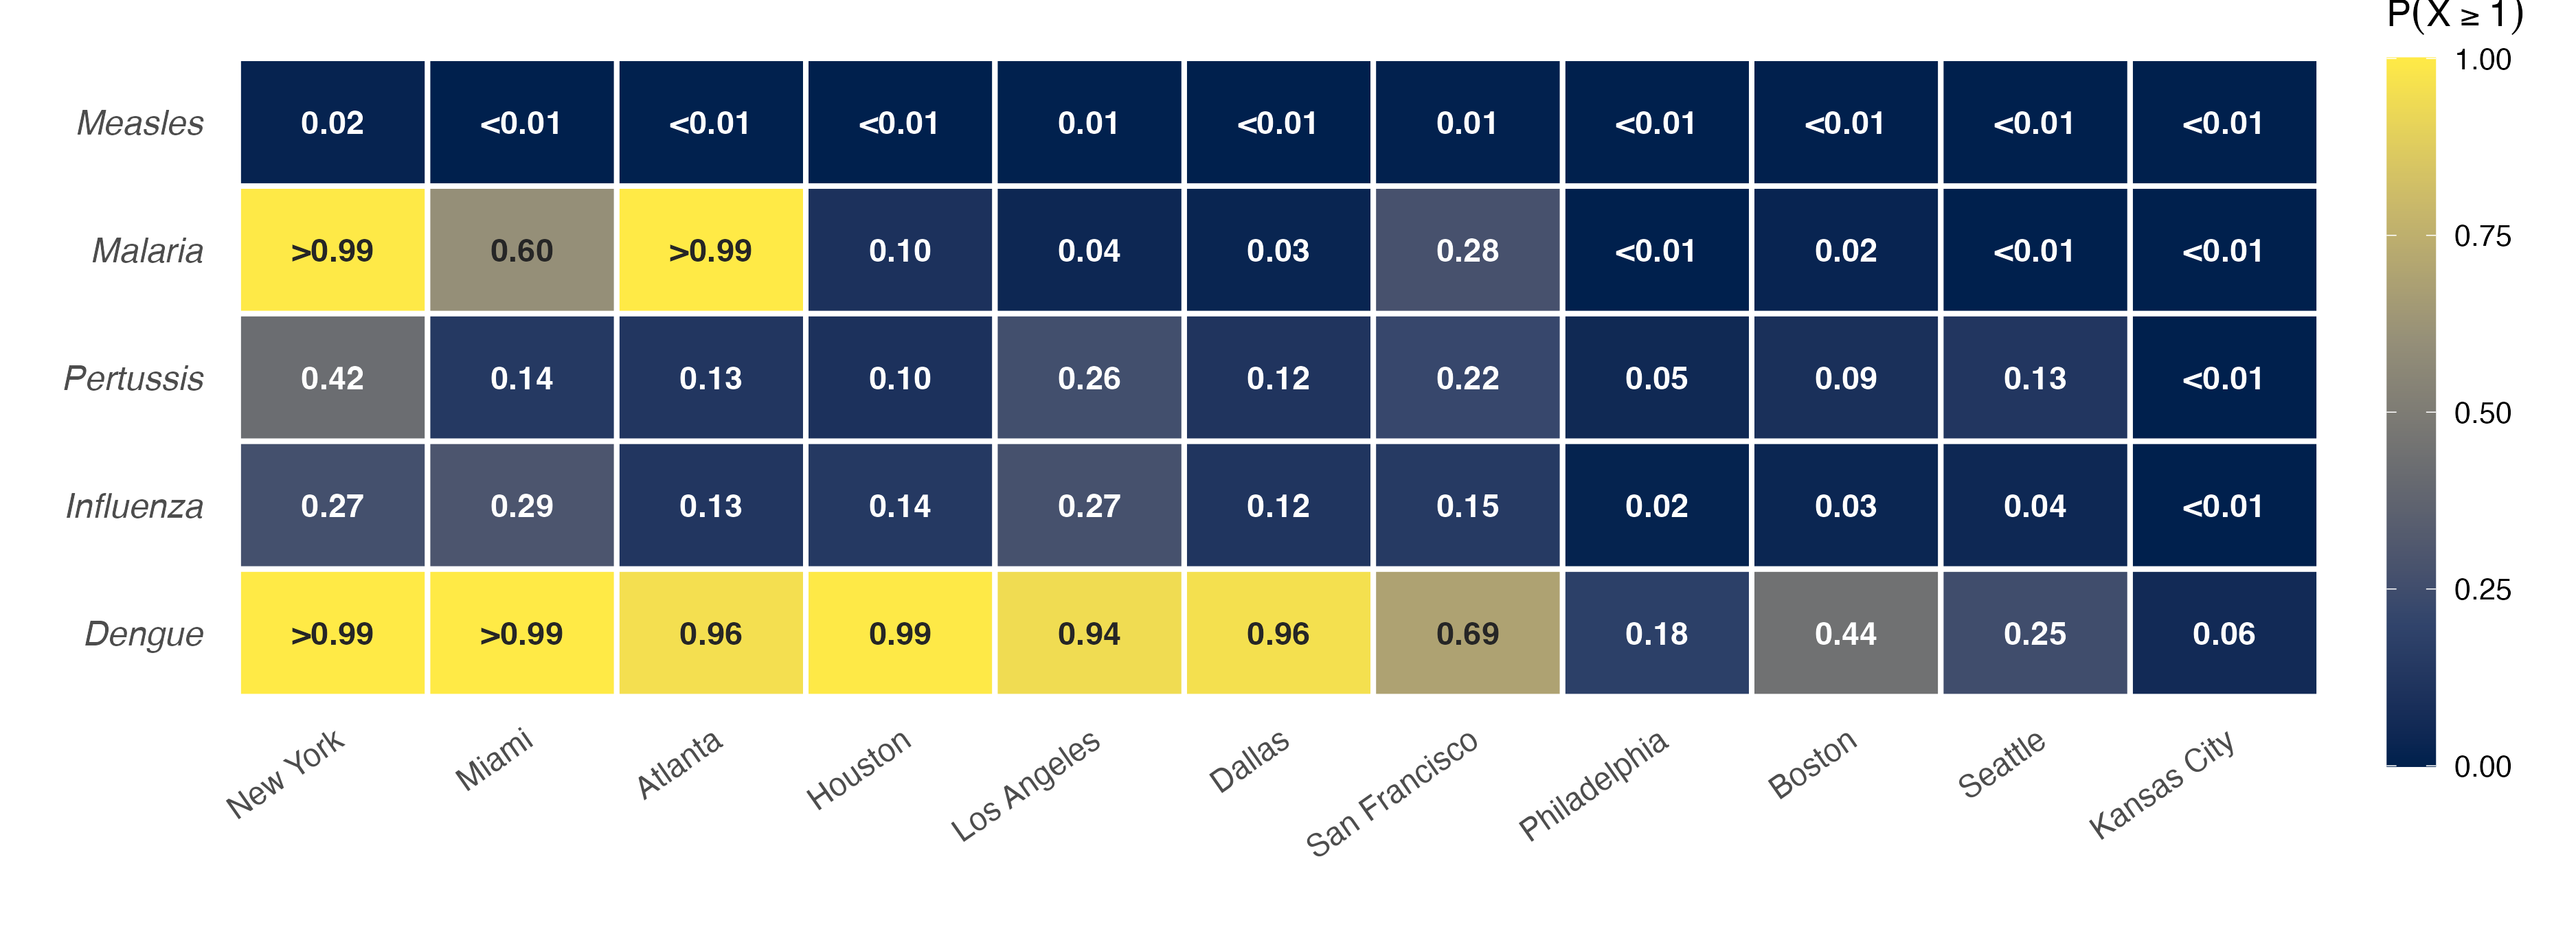
\includegraphics[width=\textwidth]{FigureS1.png}
  \caption*{\textbf{Figure S\arabic{suppfig}.}
    \textbf{Importation probability under the Baseline model (M1),
    June 2024 (no World Cup adjustment).}
    Same layout as Figure 1 in the main text. M1 represents the
    pre-tournament counterfactual: typical June travel volumes
    without the World Cup surge. Dengue $P(\geq 1) > 0.99$ is
    already present at Miami, New York, and Houston under baseline
    conditions, confirming that the World Cup amplifies but does
    not create the dengue importation threat.}
  \label{fig:s1}
\end{figure}

\newpage

% ---- Figure S2 ----------------------------------------------
\refstepcounter{suppfig}
\begin{figure}[htbp]
  \centering
  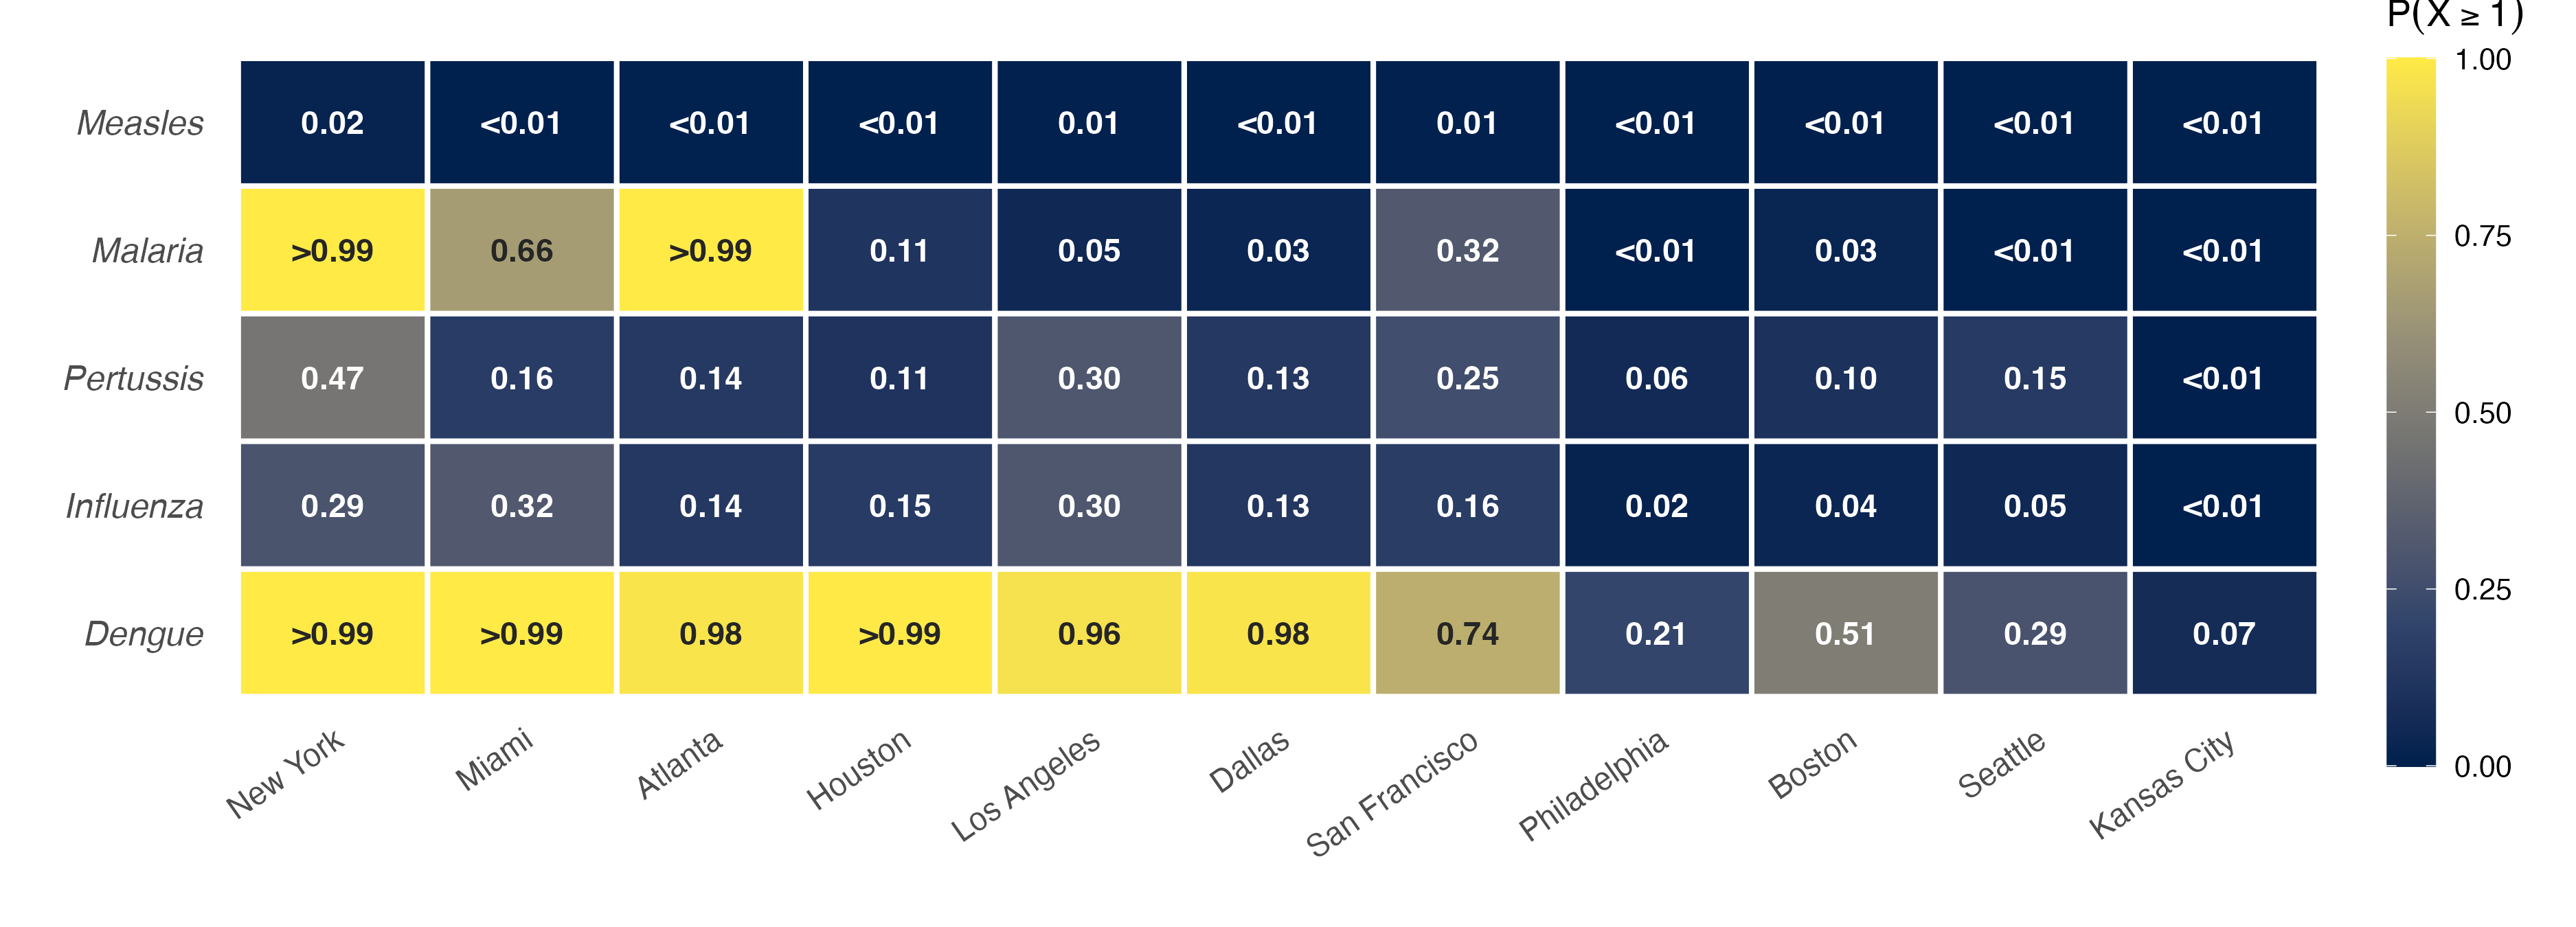
\includegraphics[width=\textwidth]{FigureS2.png}
  \caption*{\textbf{Figure S\arabic{suppfig}.}
    \textbf{Importation probability under the WC-adjusted model (M2),
    June 2026.}
    Same layout as Figure 1 in the main text. M2 applies World Cup
    growth factors to national arrivals but distributes all travel
    to US cities via T-100 routing fractions, including the fan
    increment for teams playing in Canada and Mexico. M2 values
    therefore represent a slight overestimate relative to M3 for
    US cities.}
  \label{fig:s2}
\end{figure}

\newpage

% ---- Figure S3 ----------------------------------------------
\refstepcounter{suppfig}
\begin{figure}[htbp]
  \centering
  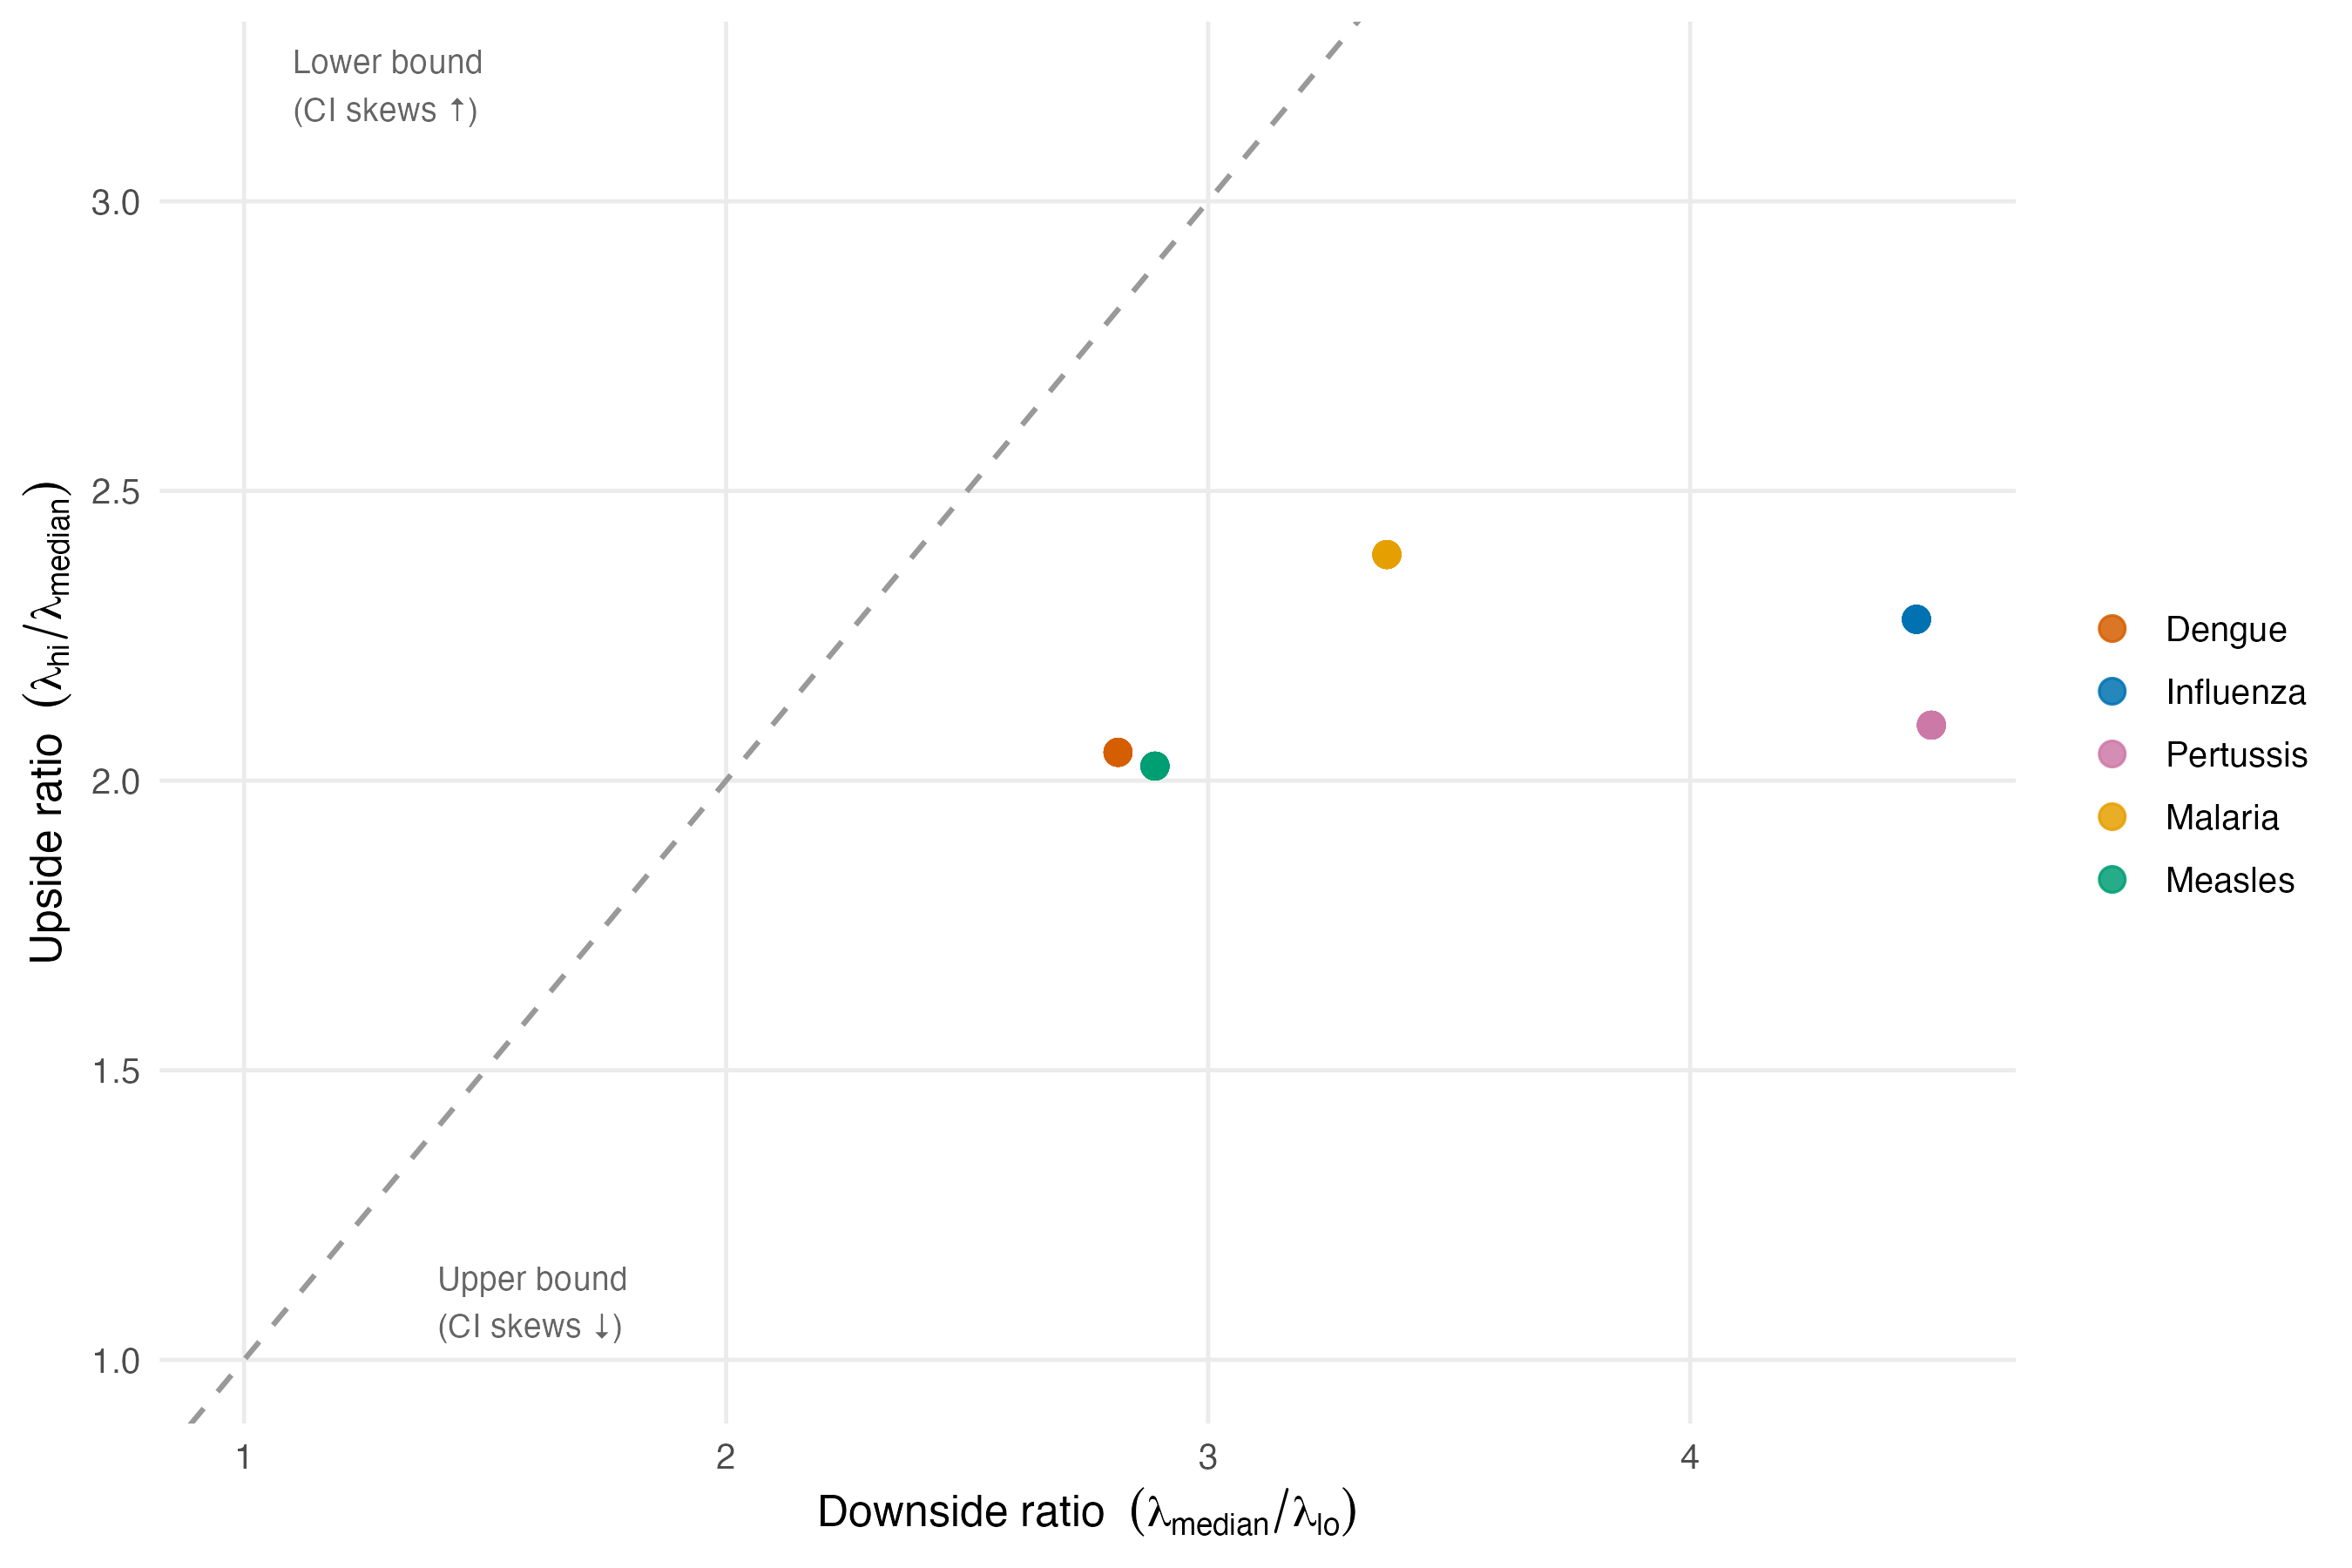
\includegraphics[width=0.85\textwidth]{FigureS3.png}
  \caption*{\textbf{Figure S\arabic{suppfig}.}
    \textbf{Direction of Monte Carlo uncertainty by disease.} Each point represents one disease--city combination. X-axis: downside ratio ($\lambda_\text{median}/\lambda_\text{lo}$), measuring how far the lower CI bound lies below the median. Y-axis: upside ratio ($\lambda_\text{hi}/\lambda_\text{median}$), measuring how far the upper CI bound lies above the median. Points above the diagonal have CIs that extend further upward; points below the diagonal have CIs that extend further downward, placing the central estimate closer to the upper plausible bound. All five diseases fall below the diagonal: uncertainty is asymmetrically larger on the  downside for every disease. Dengue and measles sit closest to the diagonal (downside ratio $\approx 2.8$), while malaria, influenza, and pertussis show larger downside ratios (4.3--4.8), indicating their medians are more conservative upper estimates.}
  \label{fig:s3}
\end{figure}

\newpage

% ---- Figure S4 ----------------------------------------------
\refstepcounter{suppfig}
\begin{figure}[htbp]
  \centering
  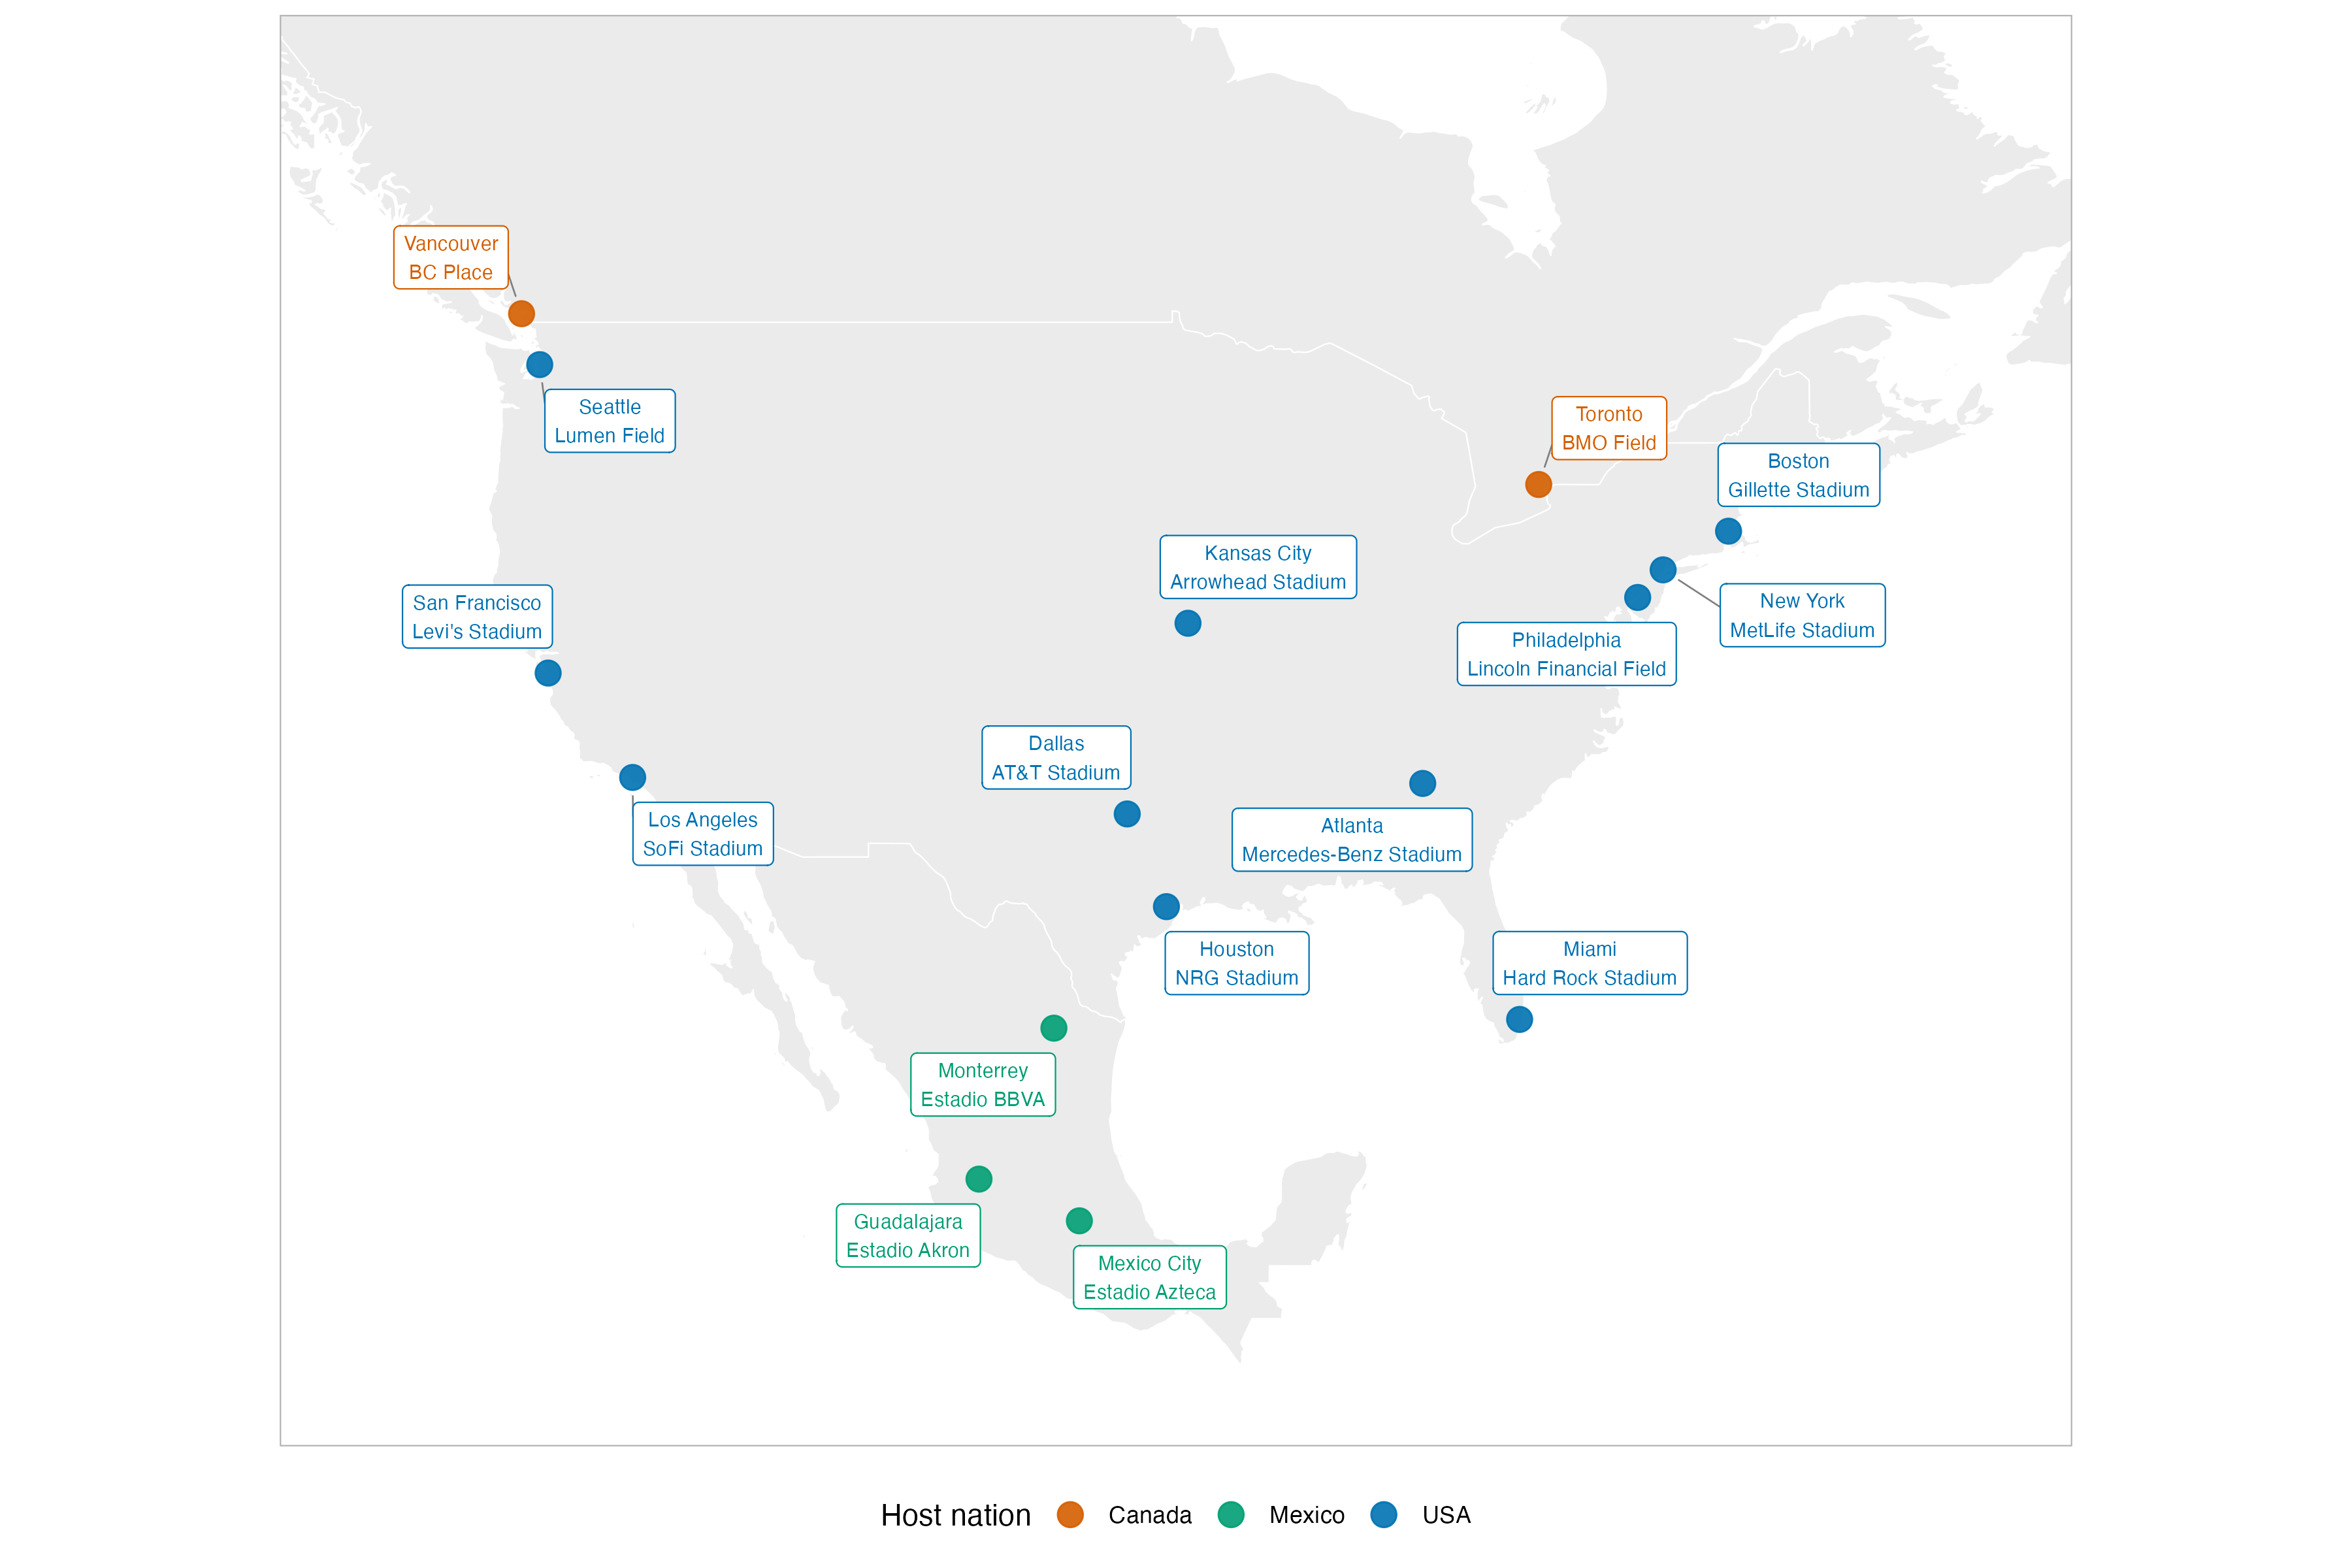
\includegraphics[width=\textwidth]{FigureS4.png}
  \caption*{\textbf{Figure S\arabic{suppfig}.}
    \textbf{Geographic distribution of the 16 FIFA World Cup 2026
    stadiums across the United States, Canada, and Mexico.}
    Colours indicate host nation. This analysis focuses on the 11
    US venues (blue); Canadian (Toronto, Vancouver) and Mexican
    (Mexico City, Monterrey, Guadalajara) venues are shown for
    context. The East Coast cluster (New York, Philadelphia, Boston)
    is the densest; Kansas City and Seattle are the most geographically
    isolated US venues.}
  \label{fig:s4}
\end{figure}

\newpage

% ---- Figure S5 ----------------------------------------------
\refstepcounter{suppfig}
\begin{figure}[htbp]
  \centering
  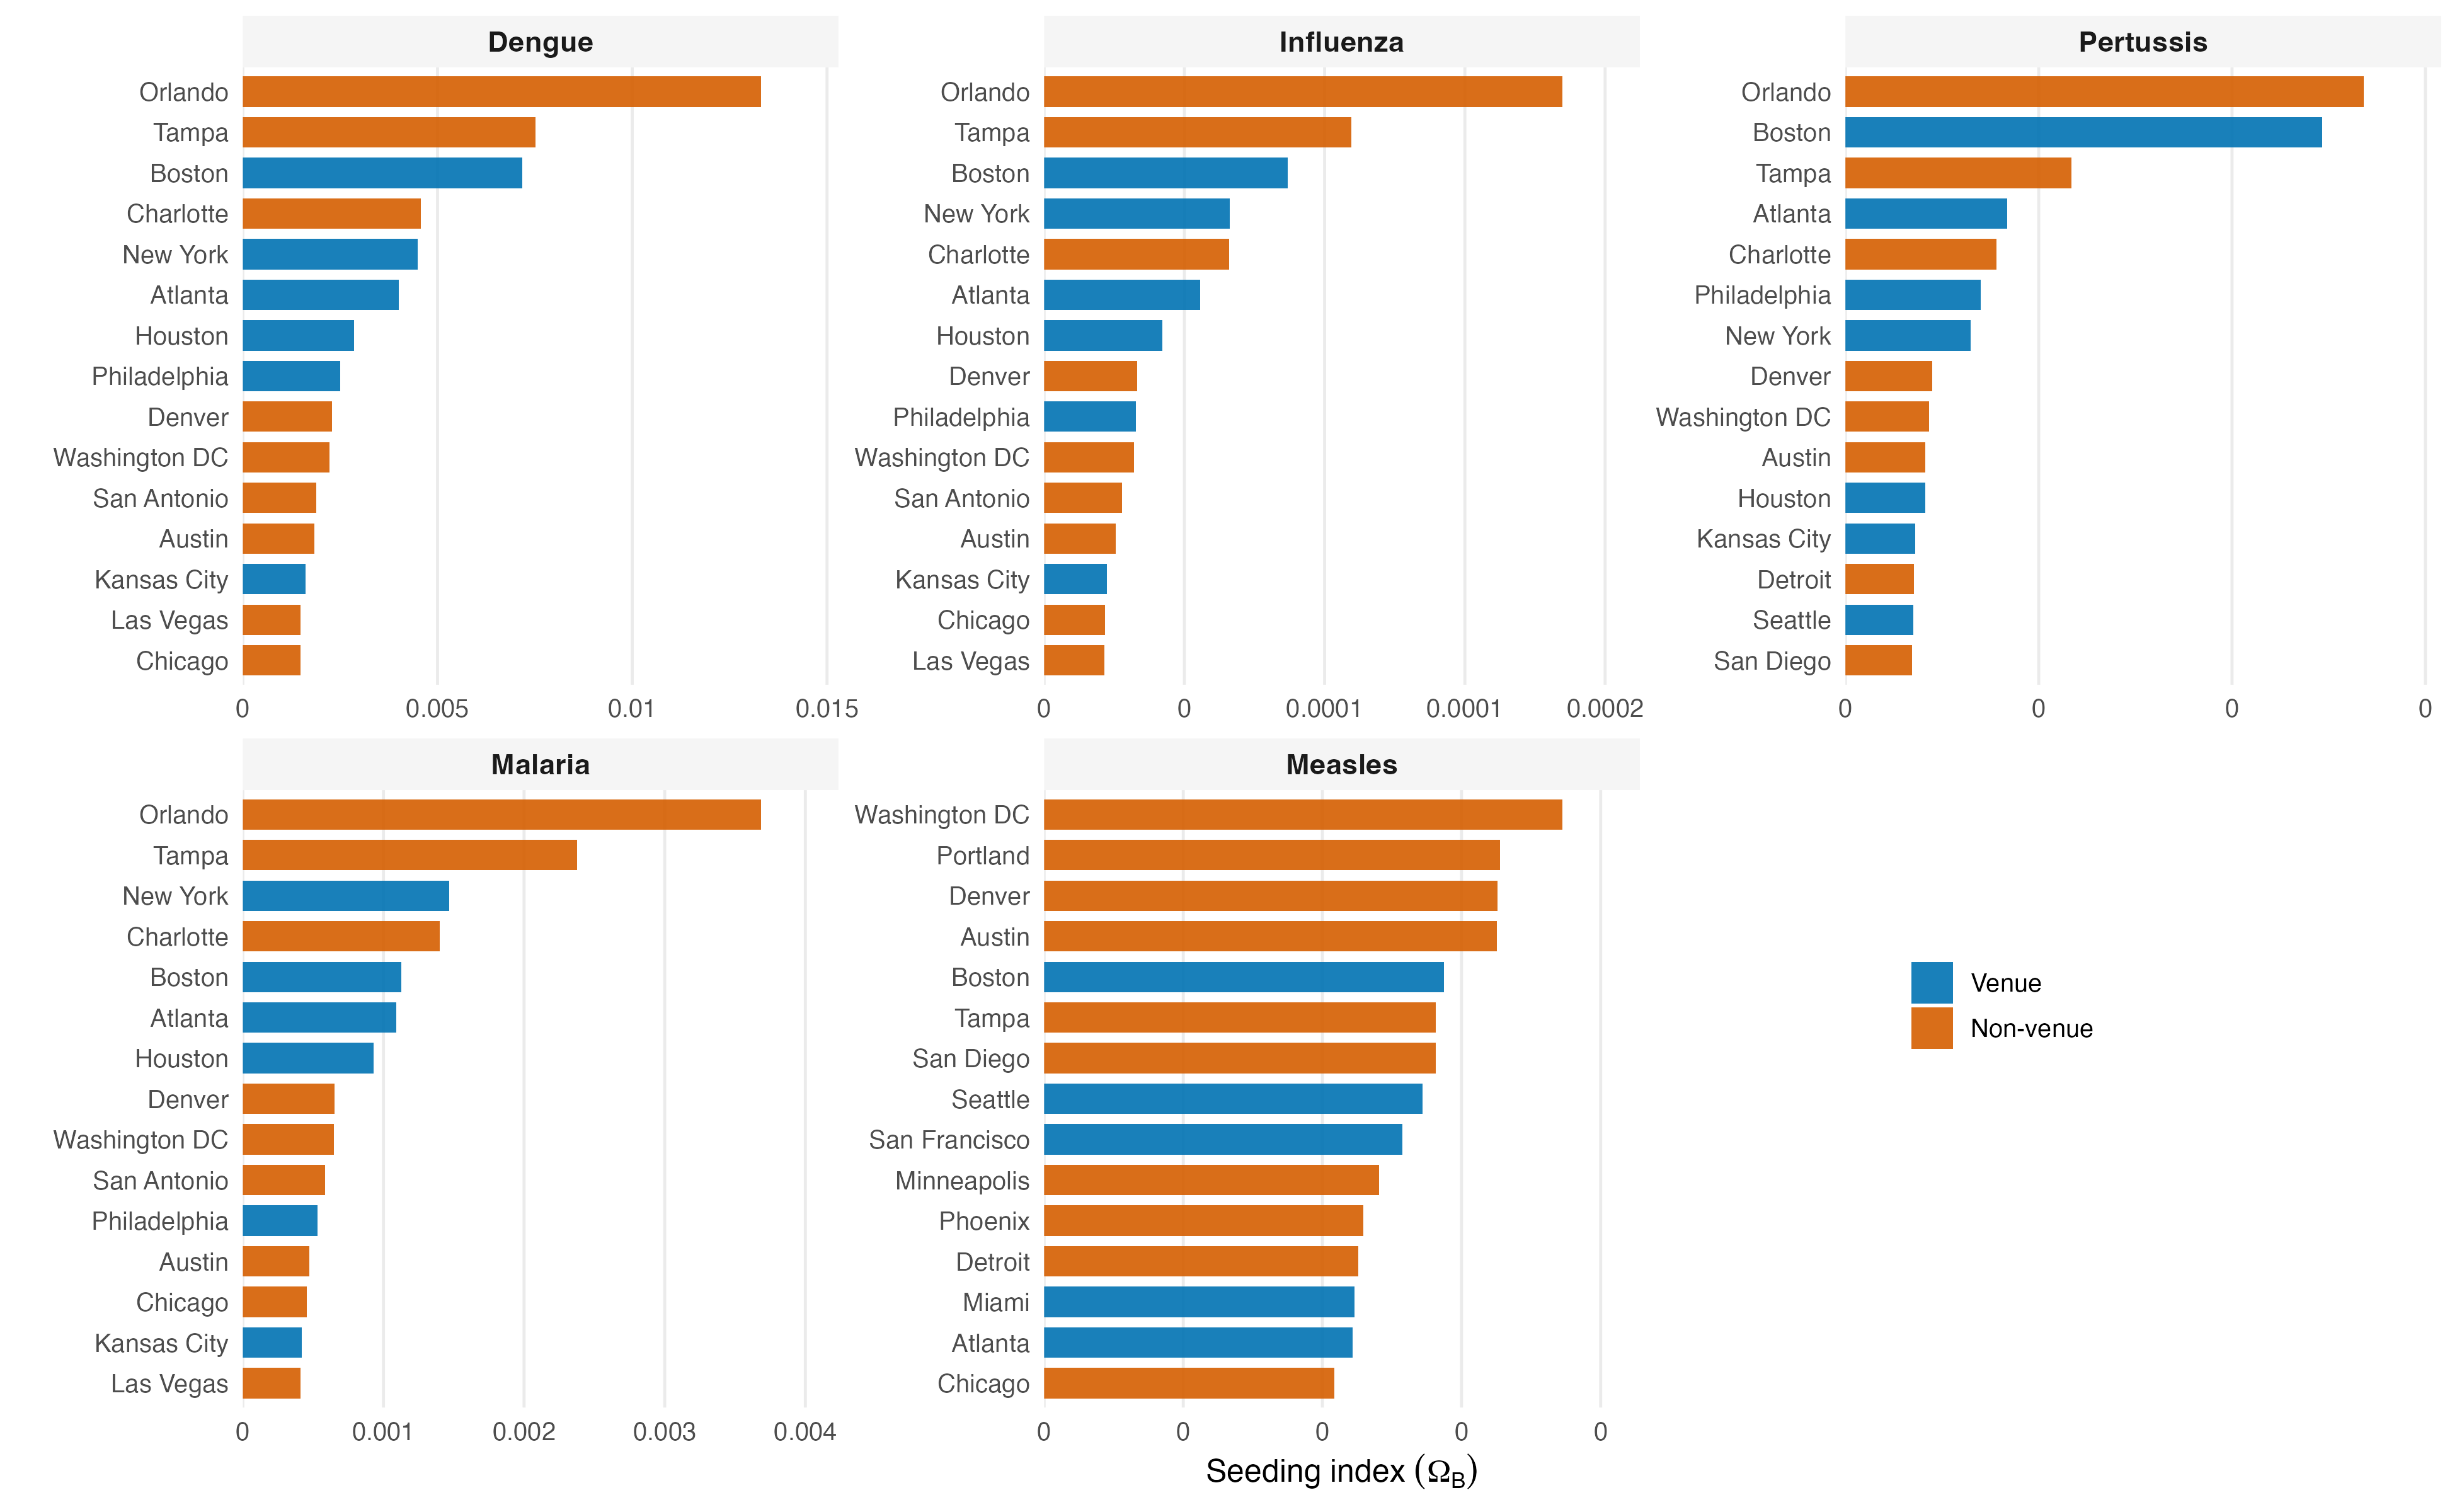
\includegraphics[width=\textwidth]{FigureS5.png}
 \caption*{\textbf{Figure S\arabic{suppfig}.}
    \textbf{Secondary seeding risk index ($\Omega^B$) for diaspora
    hub cities, by disease (Mechanism B).}
    Bars show the top 15 hub metropolitan areas per disease, ranked
    by $\Omega^B$ summed across all source countries and match venues,
    and colored by whether the hub is a World Cup host city or a
    non-host city. Hubs are the home cities to which diaspora members
    return after attending matches. $\Omega^B$ is defined only for
    source countries that are both WC-qualified and scheduled to
    play at a US venue (13 of the modeled source countries), since
    the mechanism specifically requires a match to attend; a
    country with high raw importation intensity but no US match, or
    whose risk arrives mainly via routine background travel rather
    than the match-attendance pathway, can therefore rank low or
    absent here despite dominating the raw source-country rankings
    (main text Figure 4).}
  \label{fig:s5}
\end{figure}

\newpage

% ---- Figure S6 ----------------------------------------------
\refstepcounter{suppfig}
\begin{figure}[htbp]
  \centering
  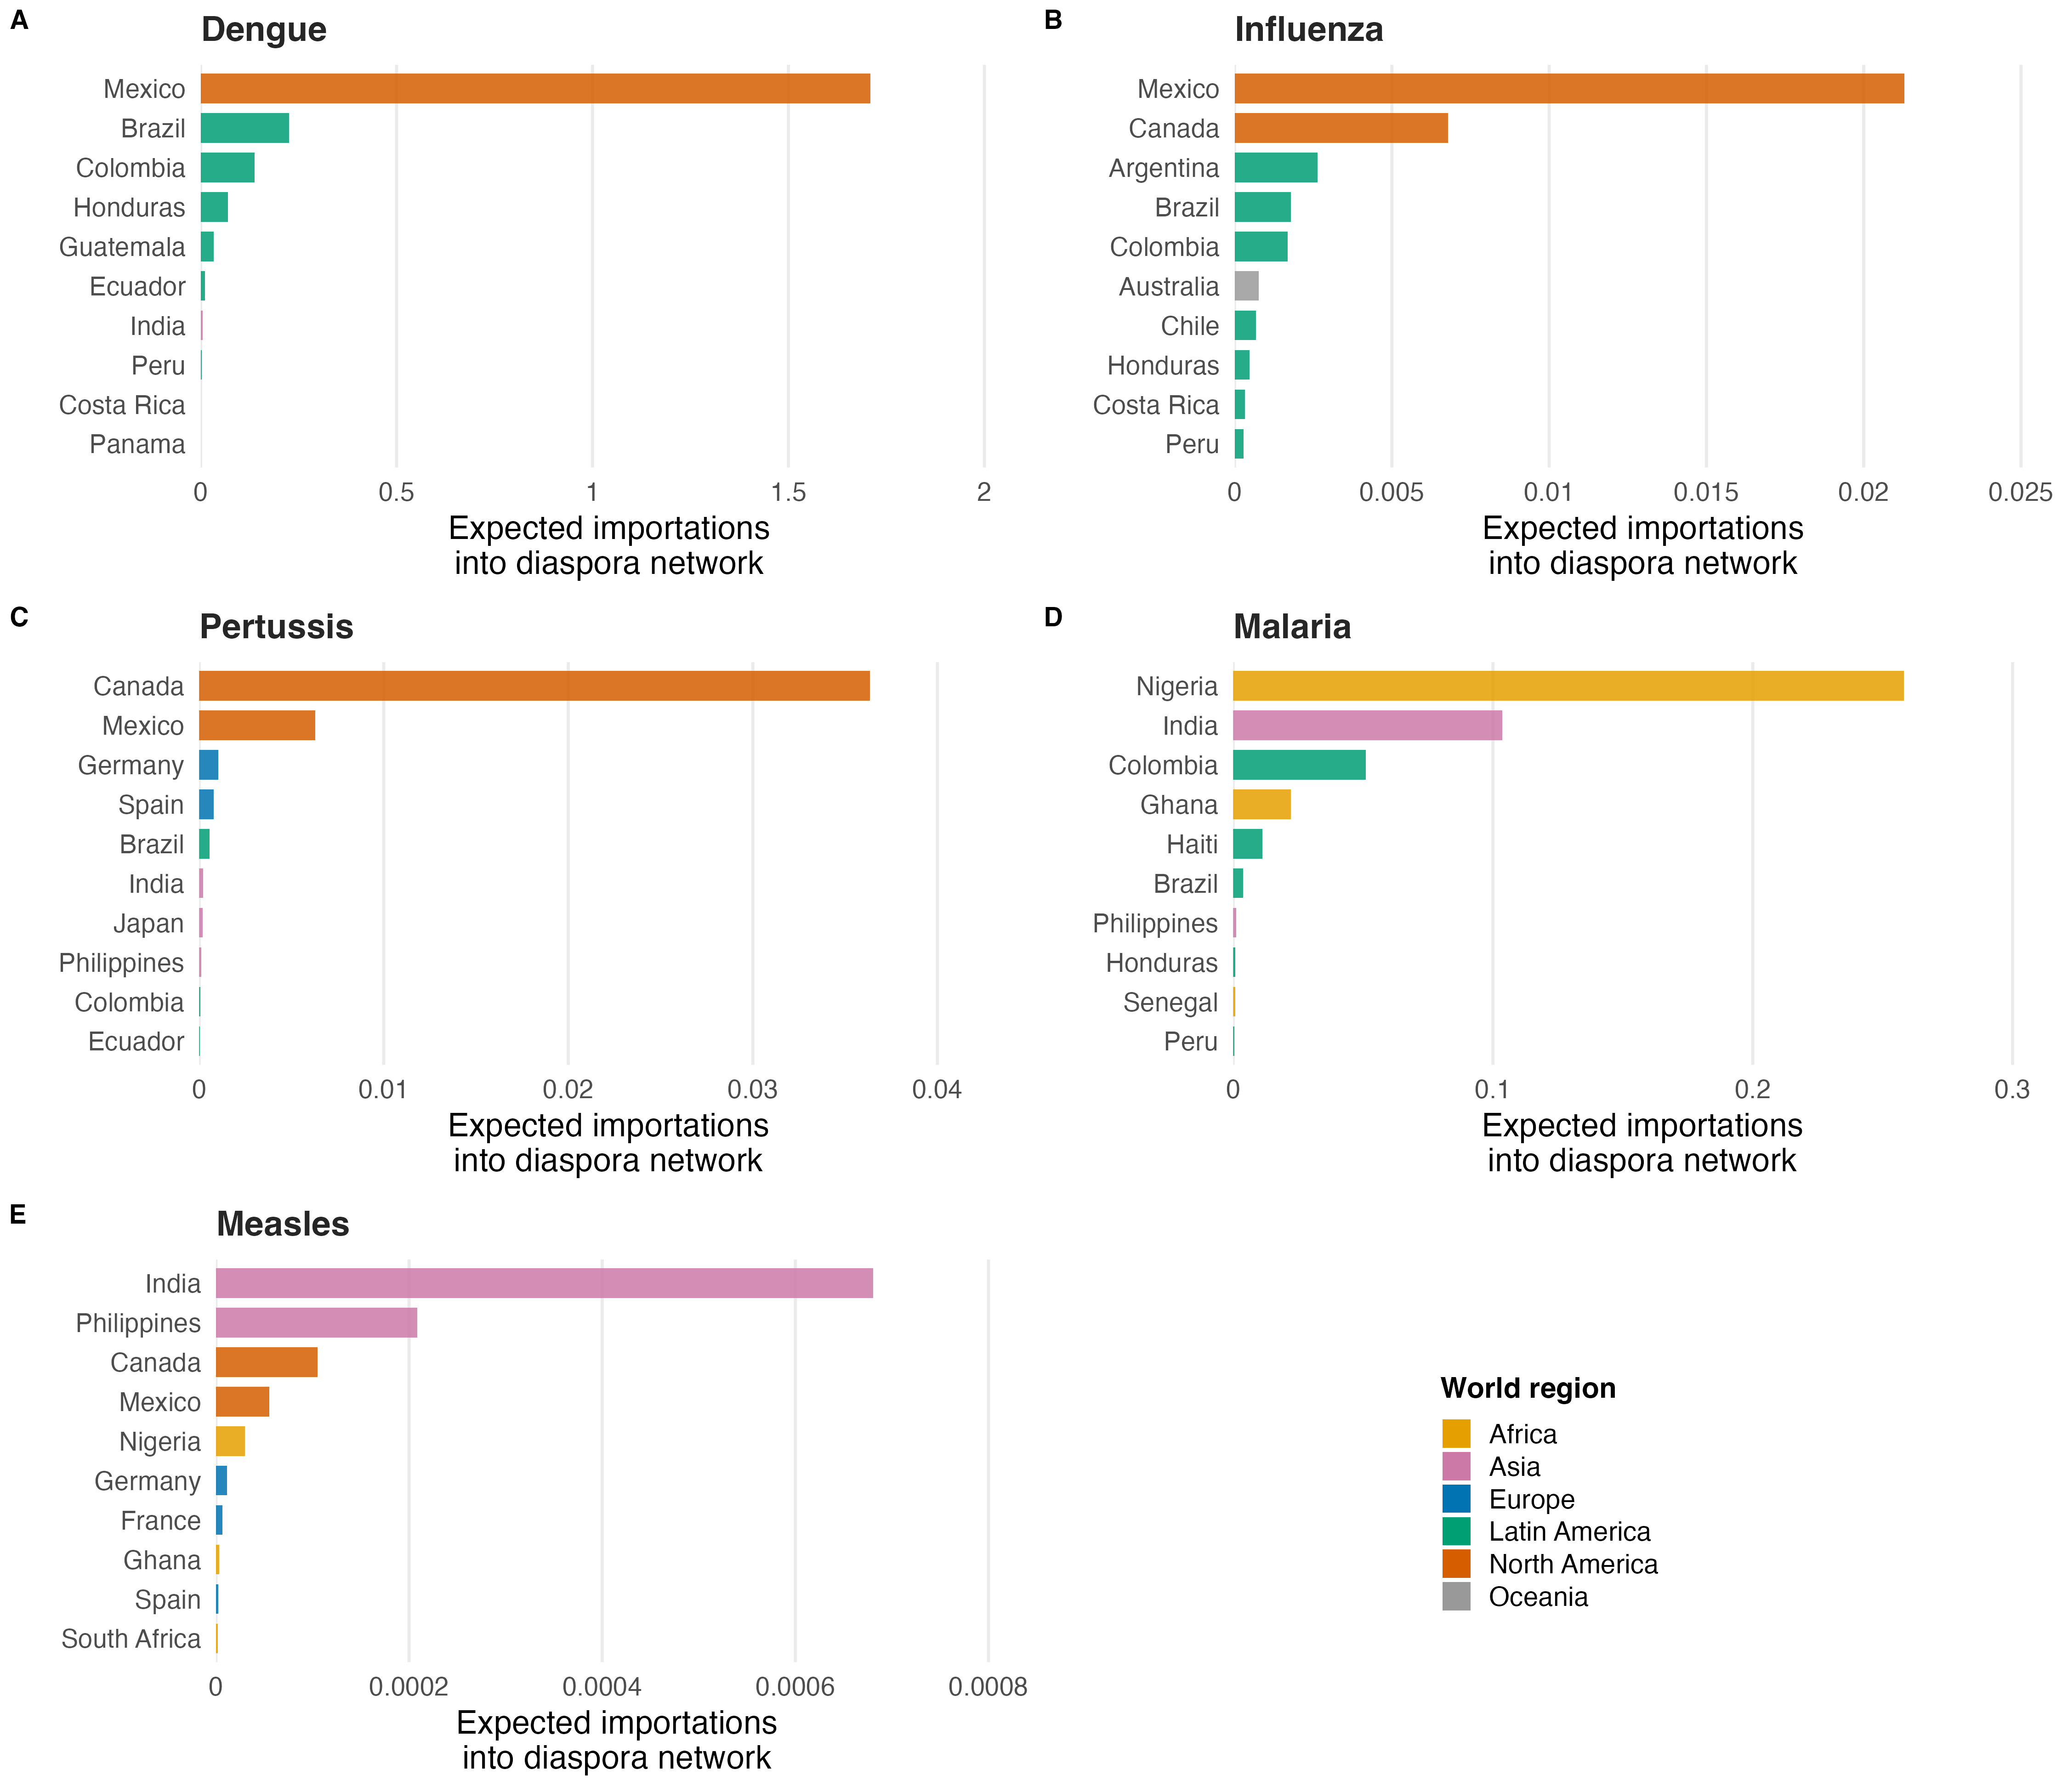
\includegraphics[width=\textwidth]{FigureS6.png}
  \caption*{\textbf{Figure S\arabic{suppfig}.}
    \textbf{Top 10 source-country contributors to diaspora-network
    importation intensity ($\Omega^A$) per disease.}
     Bars show $\Omega^A$ for each source country, summed across the
    11 host cities; colors denote world region (Canada and Mexico
    grouped as North America). The corresponding raw-$\lambda$
    ranking is shown in Figure 4 of the main text.}
  \label{fig:s6}
\end{figure}

\newpage

% ---- Figure S7 ----------------------------------------------
\refstepcounter{suppfig}
\begin{figure}[htbp]
  \centering
  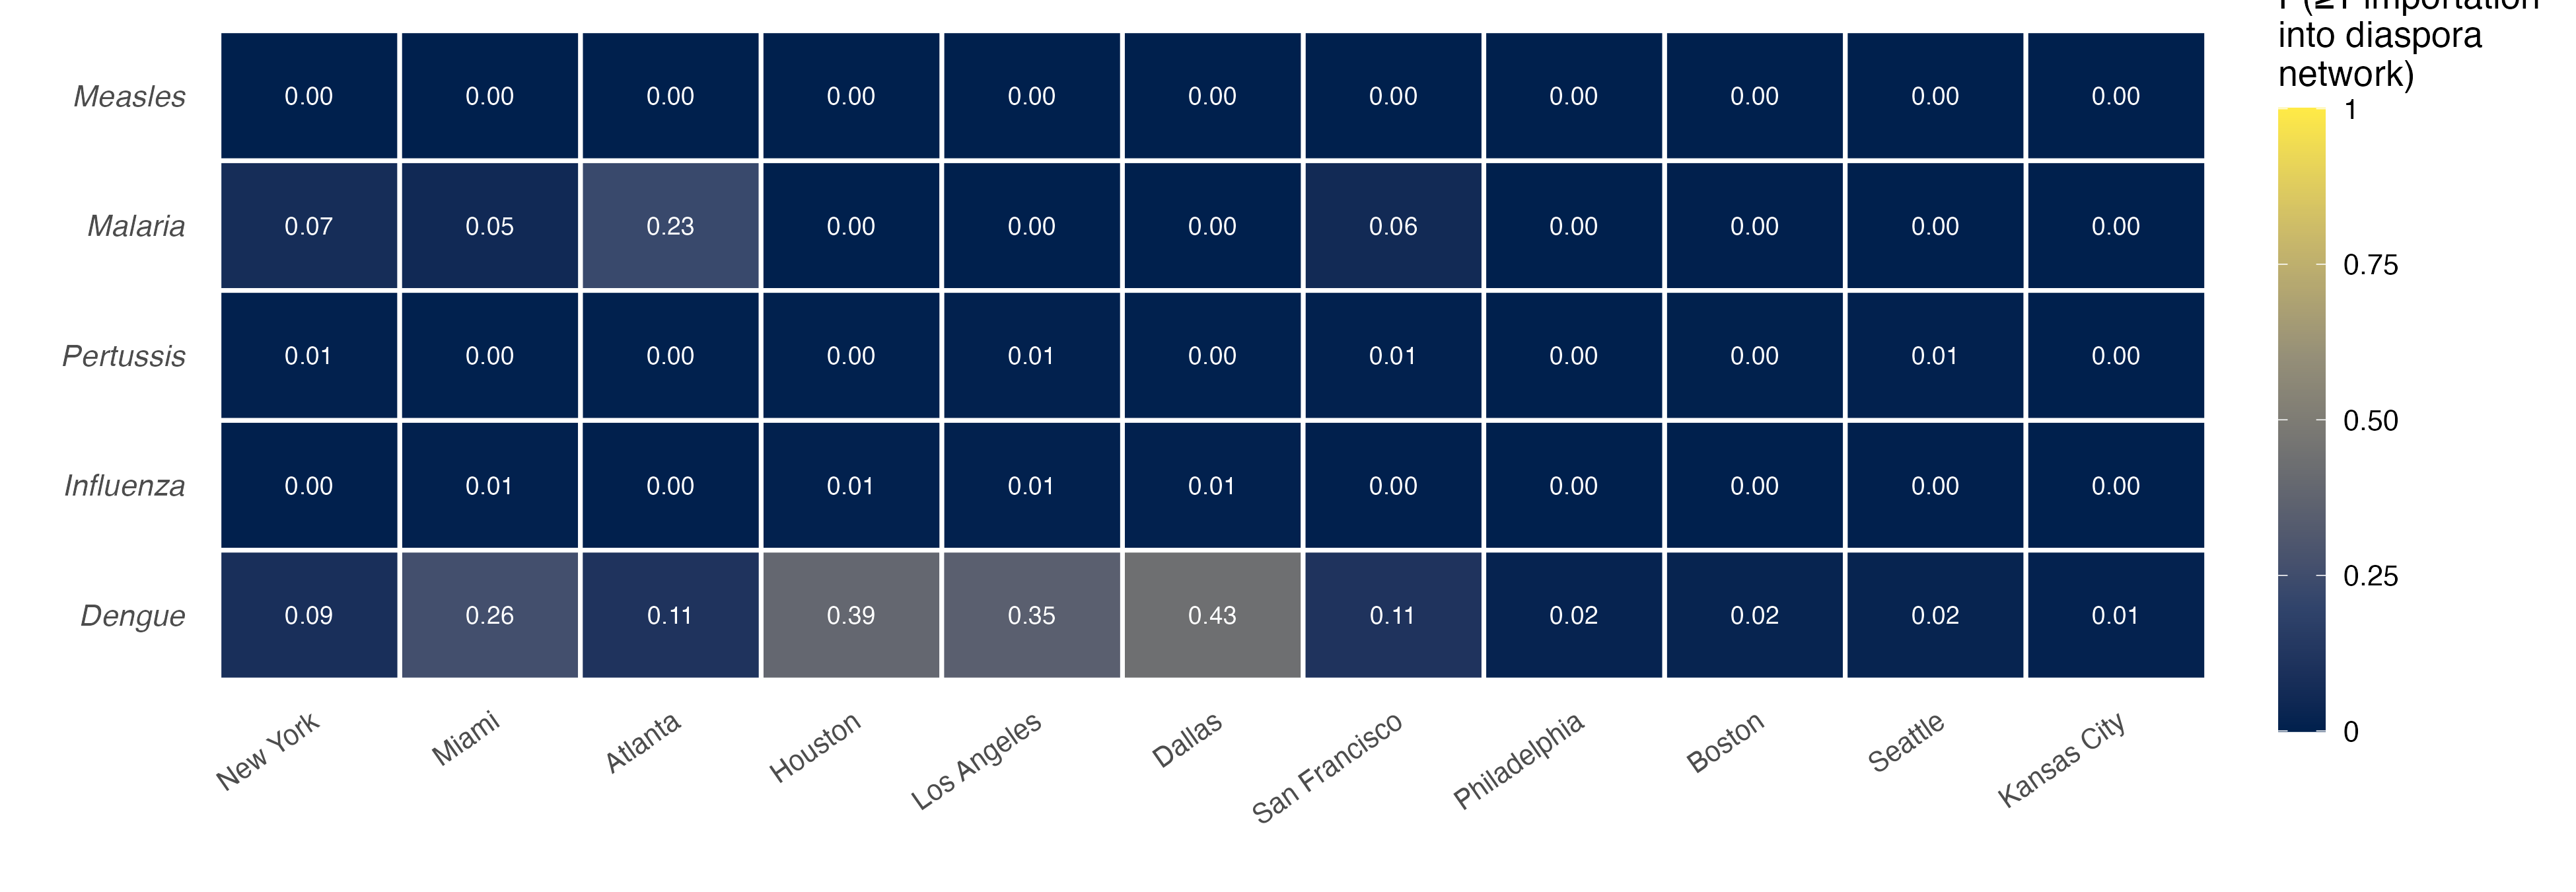
\includegraphics[width=\textwidth]{FigureS7.png}
  \caption*{\textbf{Figure S\arabic{suppfig}.}
    \textbf{Diaspora network importation probability ($P^A(\geq 1)$)
    for all five diseases at 11 US host cities.}
    Cells show $P^A(\geq 1)_{v,d}$, the probability that at least one
    imported case enters a co-national diaspora network at each host
    city. The dengue and malaria rows correspond to Panel A of
    Figure 5 in the main text.}
  \label{fig:s7b}
\end{figure}

\newpage

% ---- Figure S8 ----------------------------------------------
\refstepcounter{suppfig}
\begin{figure}[htbp]
  \centering
  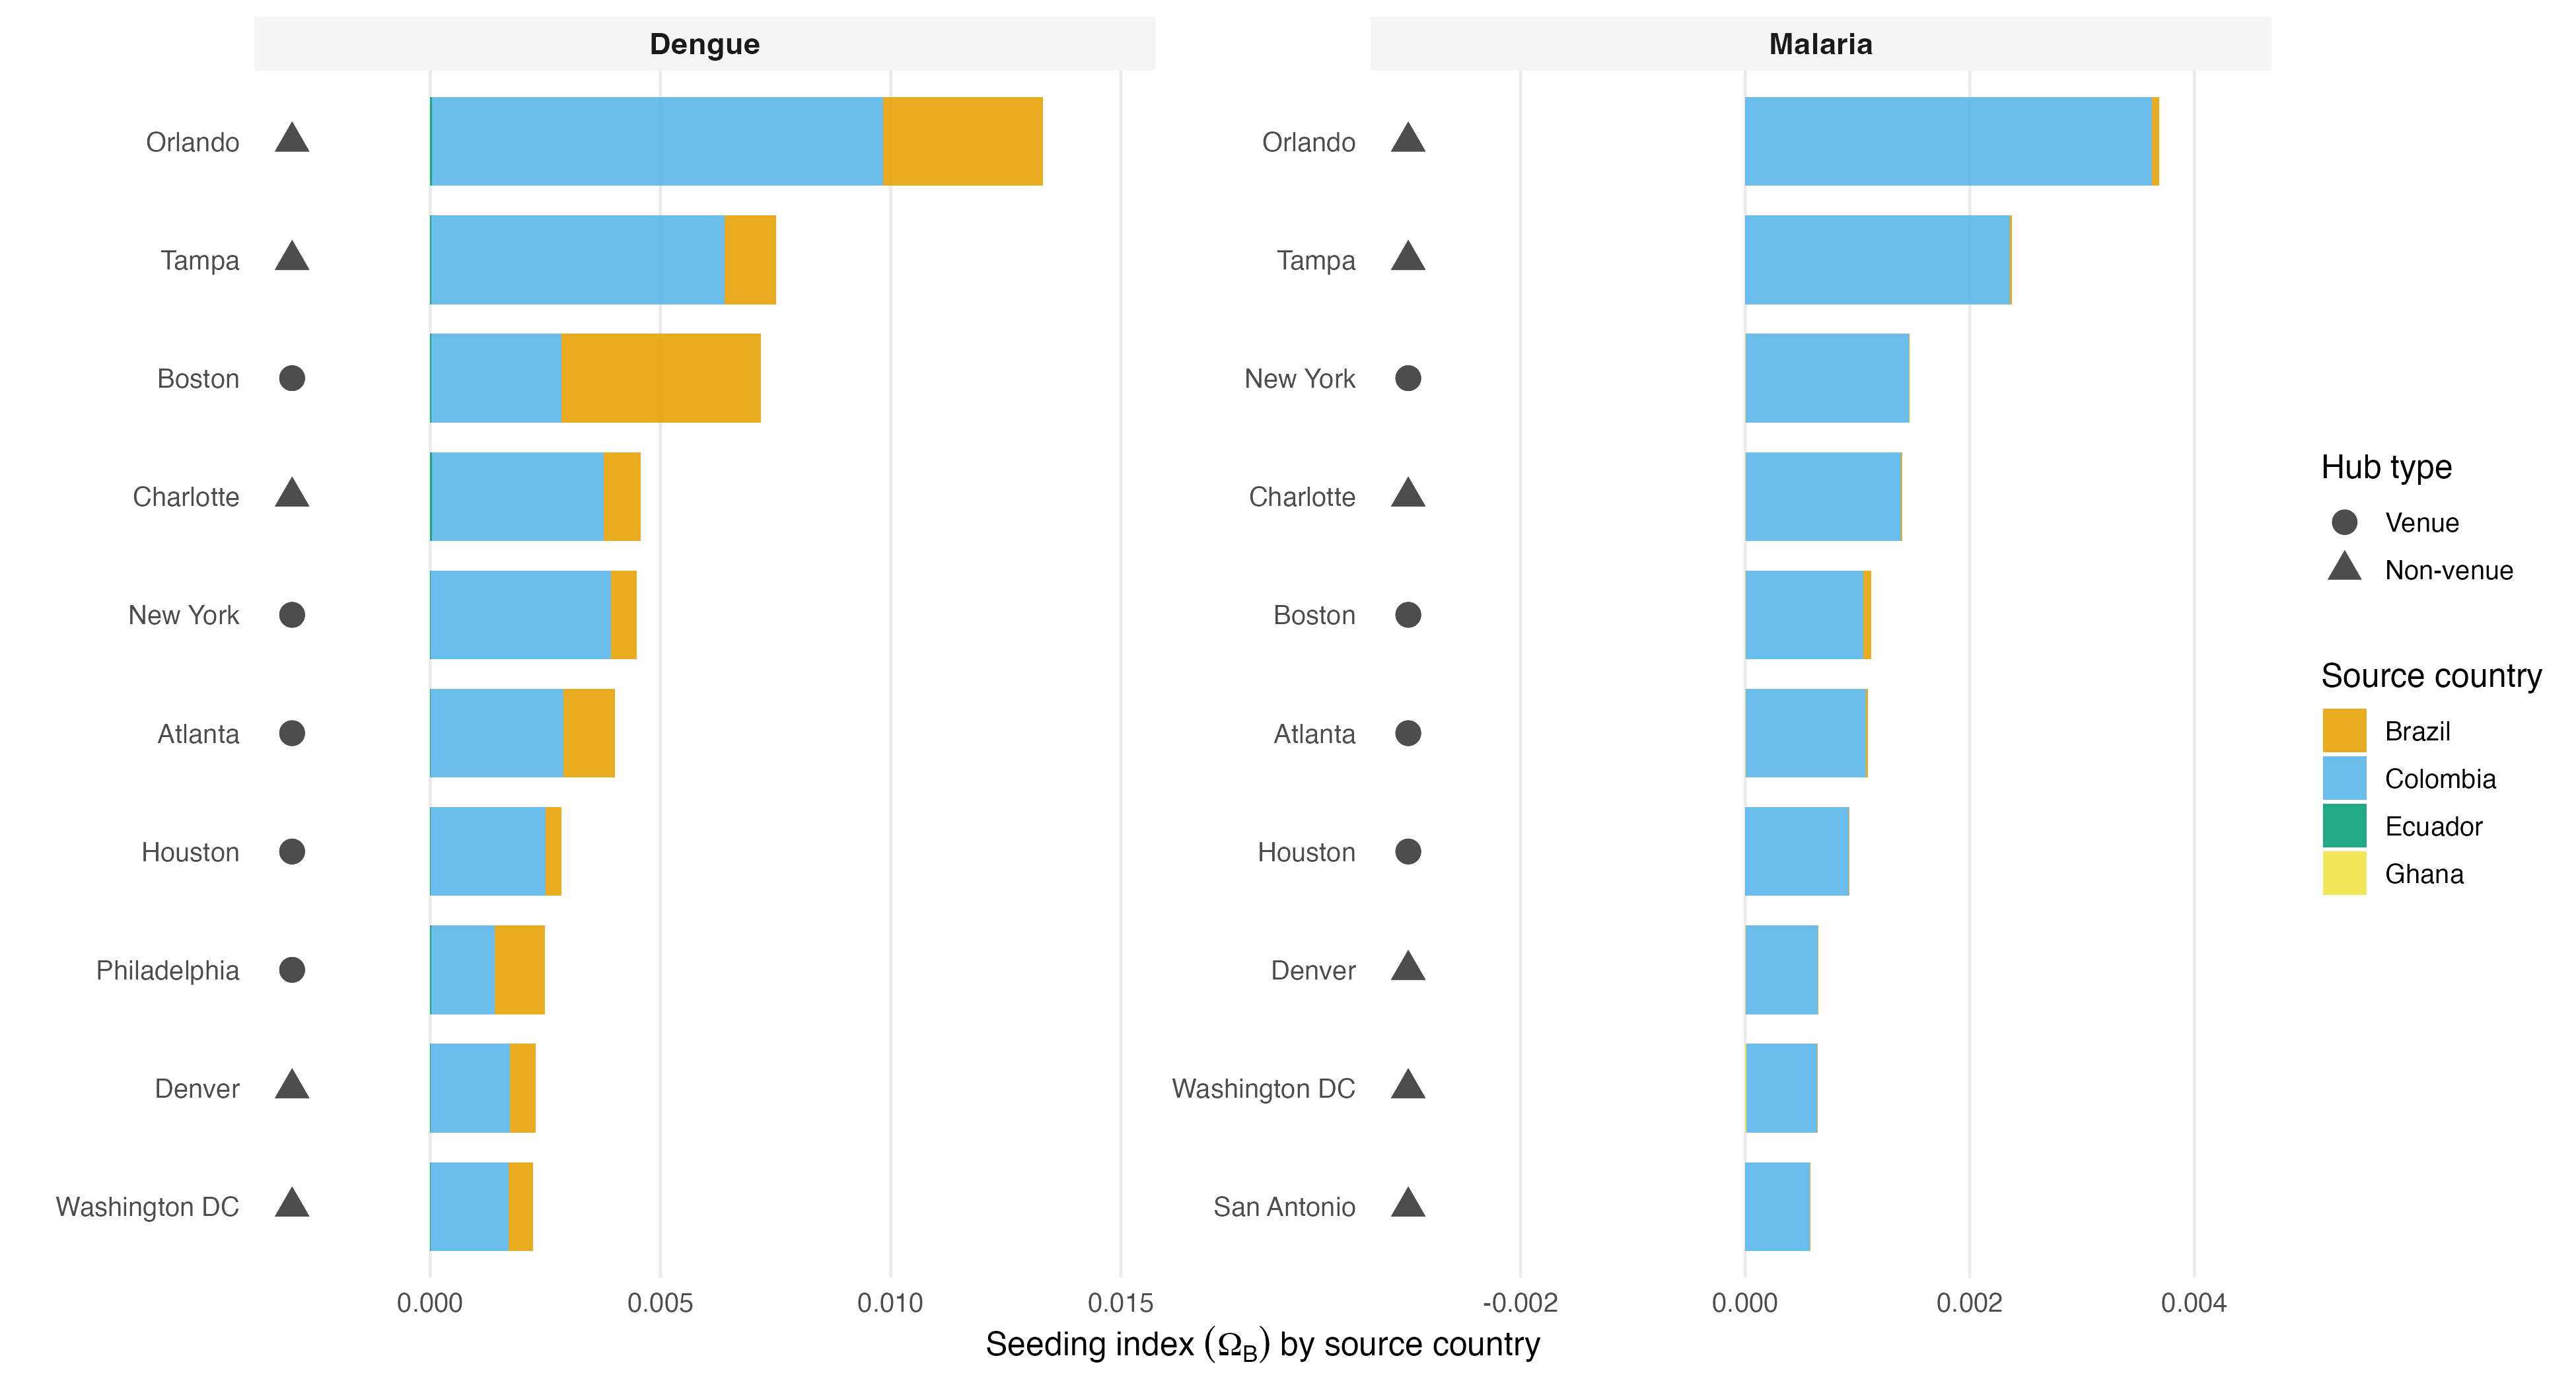
\includegraphics[width=\textwidth]{FigureS8.png}
  \caption*{\textbf{Figure S\arabic{suppfig}.} \textbf{Source-country contributions to Mechanism B secondary seeding index ($\Omega^B$) for dengue and malaria.}
      Bars show the source-country contributions to $\Omega^B$ at
      each of the top hub cities per disease, ranked by total
      $\Omega^B$. Dot shape distinguishes World Cup venue cities
      (circle) from non-venue metropolitan areas (triangle). Because
      Mechanism B specifically requires a diaspora member to travel
      to a match involving their home country, it is restricted to
      the subset of source countries that are both WC-qualified and
      scheduled to play at a US venue; for both dengue and malaria,
      Colombia and Brazil are the only such countries with incidence
      high enough to register, so they drive secondary seeding at
      every top hub. Countries with much larger raw arrival
      intensities for these diseases (e.g., Nigeria for malaria)
      do not appear here because their risk arrives via routine
      background travel to cities where their team is not playing,
      a pathway Mechanism A already captures but that falls outside
      Mechanism B's match-attendance pathway (see main text Limitations and Appendix B.4).
      Non-venue hubs (Orlando, Tampa, Charlotte, Denver,
      Washington, DC) rank alongside host cities because of their
      large Colombian and Brazilian diaspora concentrations.}
  \label{fig:s8}
\end{figure}

\newpage

% =============================================================
% REFERENCES
% =============================================================
\bibliographystyle{vancouver}
\bibliography{references_IJID}

\end{document}
